% figures.tex -- Figures collected after the tables
\section*{Figures}

\begin{center}
\begin{minipage}{\linewidth}
\captionsetup{type=figure,hypcap=false}
  \centering
  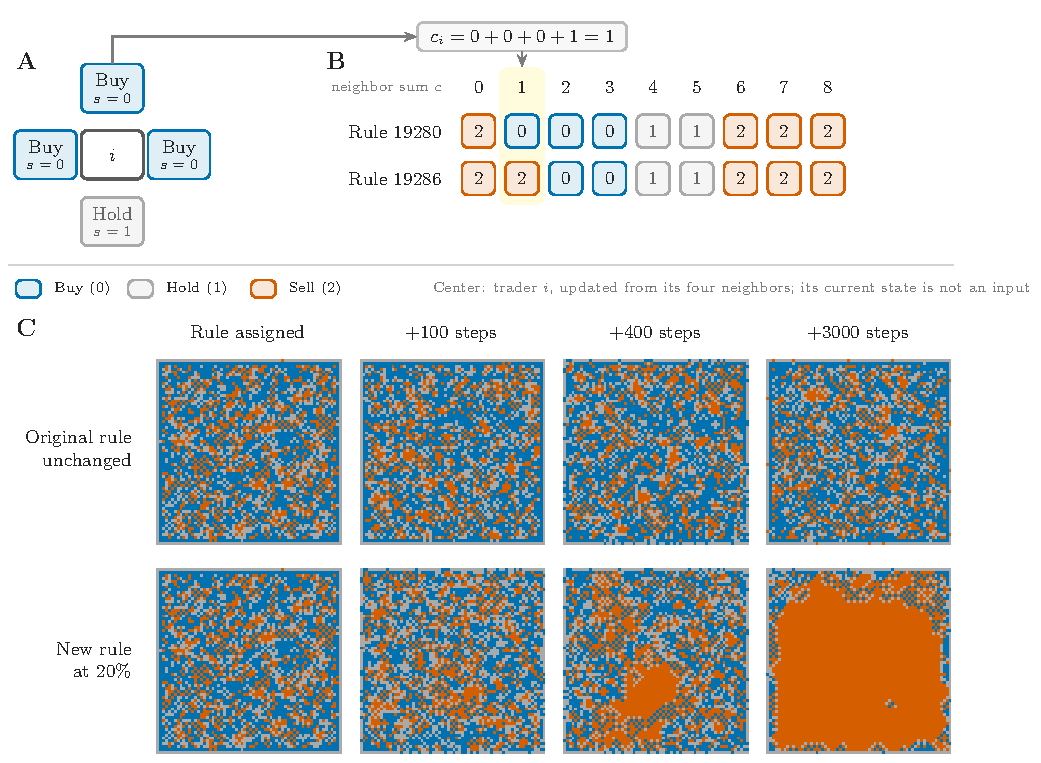
\includegraphics[width=0.95\linewidth]{figs/Fig1-RuleQuench.pdf}
  \caption{Changing the decision rule caused initially identical markets to develop
differently. Fifty starting markets were simulated on a $64\times64$ grid
for 1,000 steps before the rule change and 3,000 steps afterward. Each
comparison market kept the original rule at the same selected sites.
\textbf{(A)}~Median price divided by its value when the rule changed; bands
mark the interquartile range. \textbf{(B)}~Median fraction of interior
traders in Sell; the horizontal line marks one-half. \textbf{(C)}~Snapshots
of decisions for seed 12, the $f=0.20$ pair nearest the median difference in
peak Sell fraction between changed and unchanged markets. Blue, gray, and
orange cells denote Buy, Hold, and Sell. Rows follow the two markets from
their common state when the rule was assigned through 3,000 steps. All
paired markets were identical before the vertical line marking the rule
change.}
  \label{fig:rule-quench}
\end{minipage}
\end{center}

\clearpage

\begin{center}
\begin{minipage}{\linewidth}
\captionsetup{type=figure,hypcap=false}
  \centering
  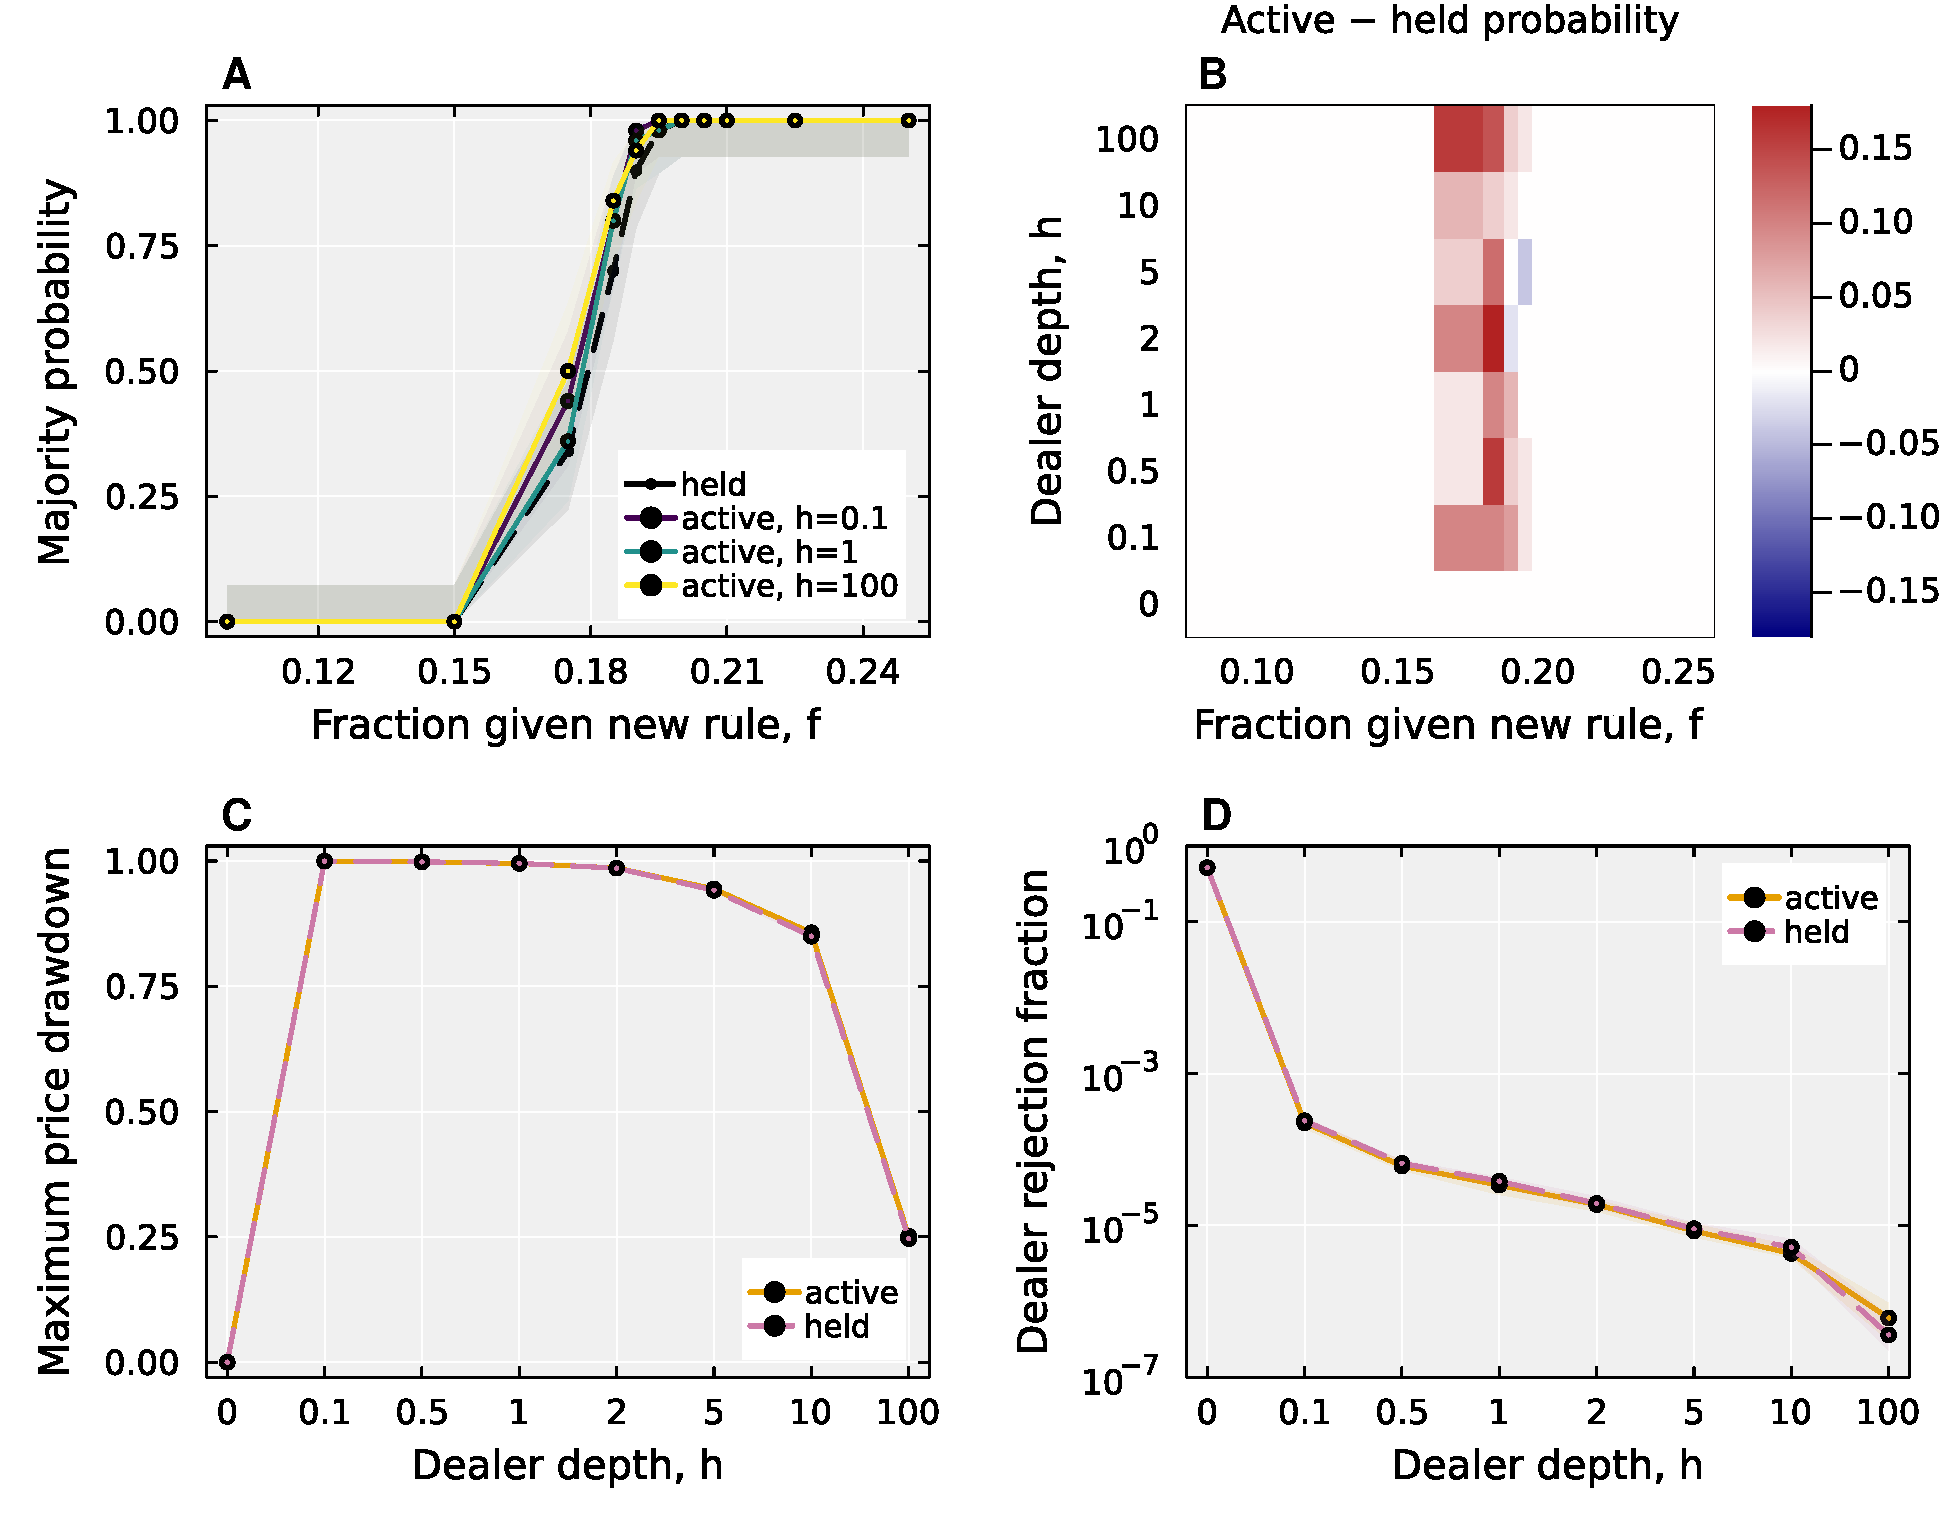
\includegraphics[width=0.97\linewidth]{figs/Fig2-ReservoirQuench.pdf}
  \caption{Changing decision rules while varying how much the dealer could buy and
sell. \textbf{(A)}~Probability of a Sell majority with edge traders kept in
Hold and with those traders responding to price at selected dealer
capacities. These conditions are labeled held boundary and endogenous
boundary, respectively. Bands are 95\% Wilson intervals over 50 starting
markets. \textbf{(B)}~Difference in majority probability between the
condition with edge traders responding to price and the condition with them
kept in Hold, across all capacities. \textbf{(C)}~Median maximum drawdown at
$f=0.20$; bands mark the interquartile range. \textbf{(D)}~Median fraction
of orders backed by trader cash or shares that the dealer rejected at
$f=0.20$. Capacity $h=10$ appears as a dashed overlay in (A) and a separate
capacity in (B--D); it matched $h=\infty$ exactly.}
  \label{fig:reservoir}
\end{minipage}
\end{center}

\clearpage

\begin{center}
\begin{minipage}{\linewidth}
\captionsetup{type=figure,hypcap=false}
  \centering
  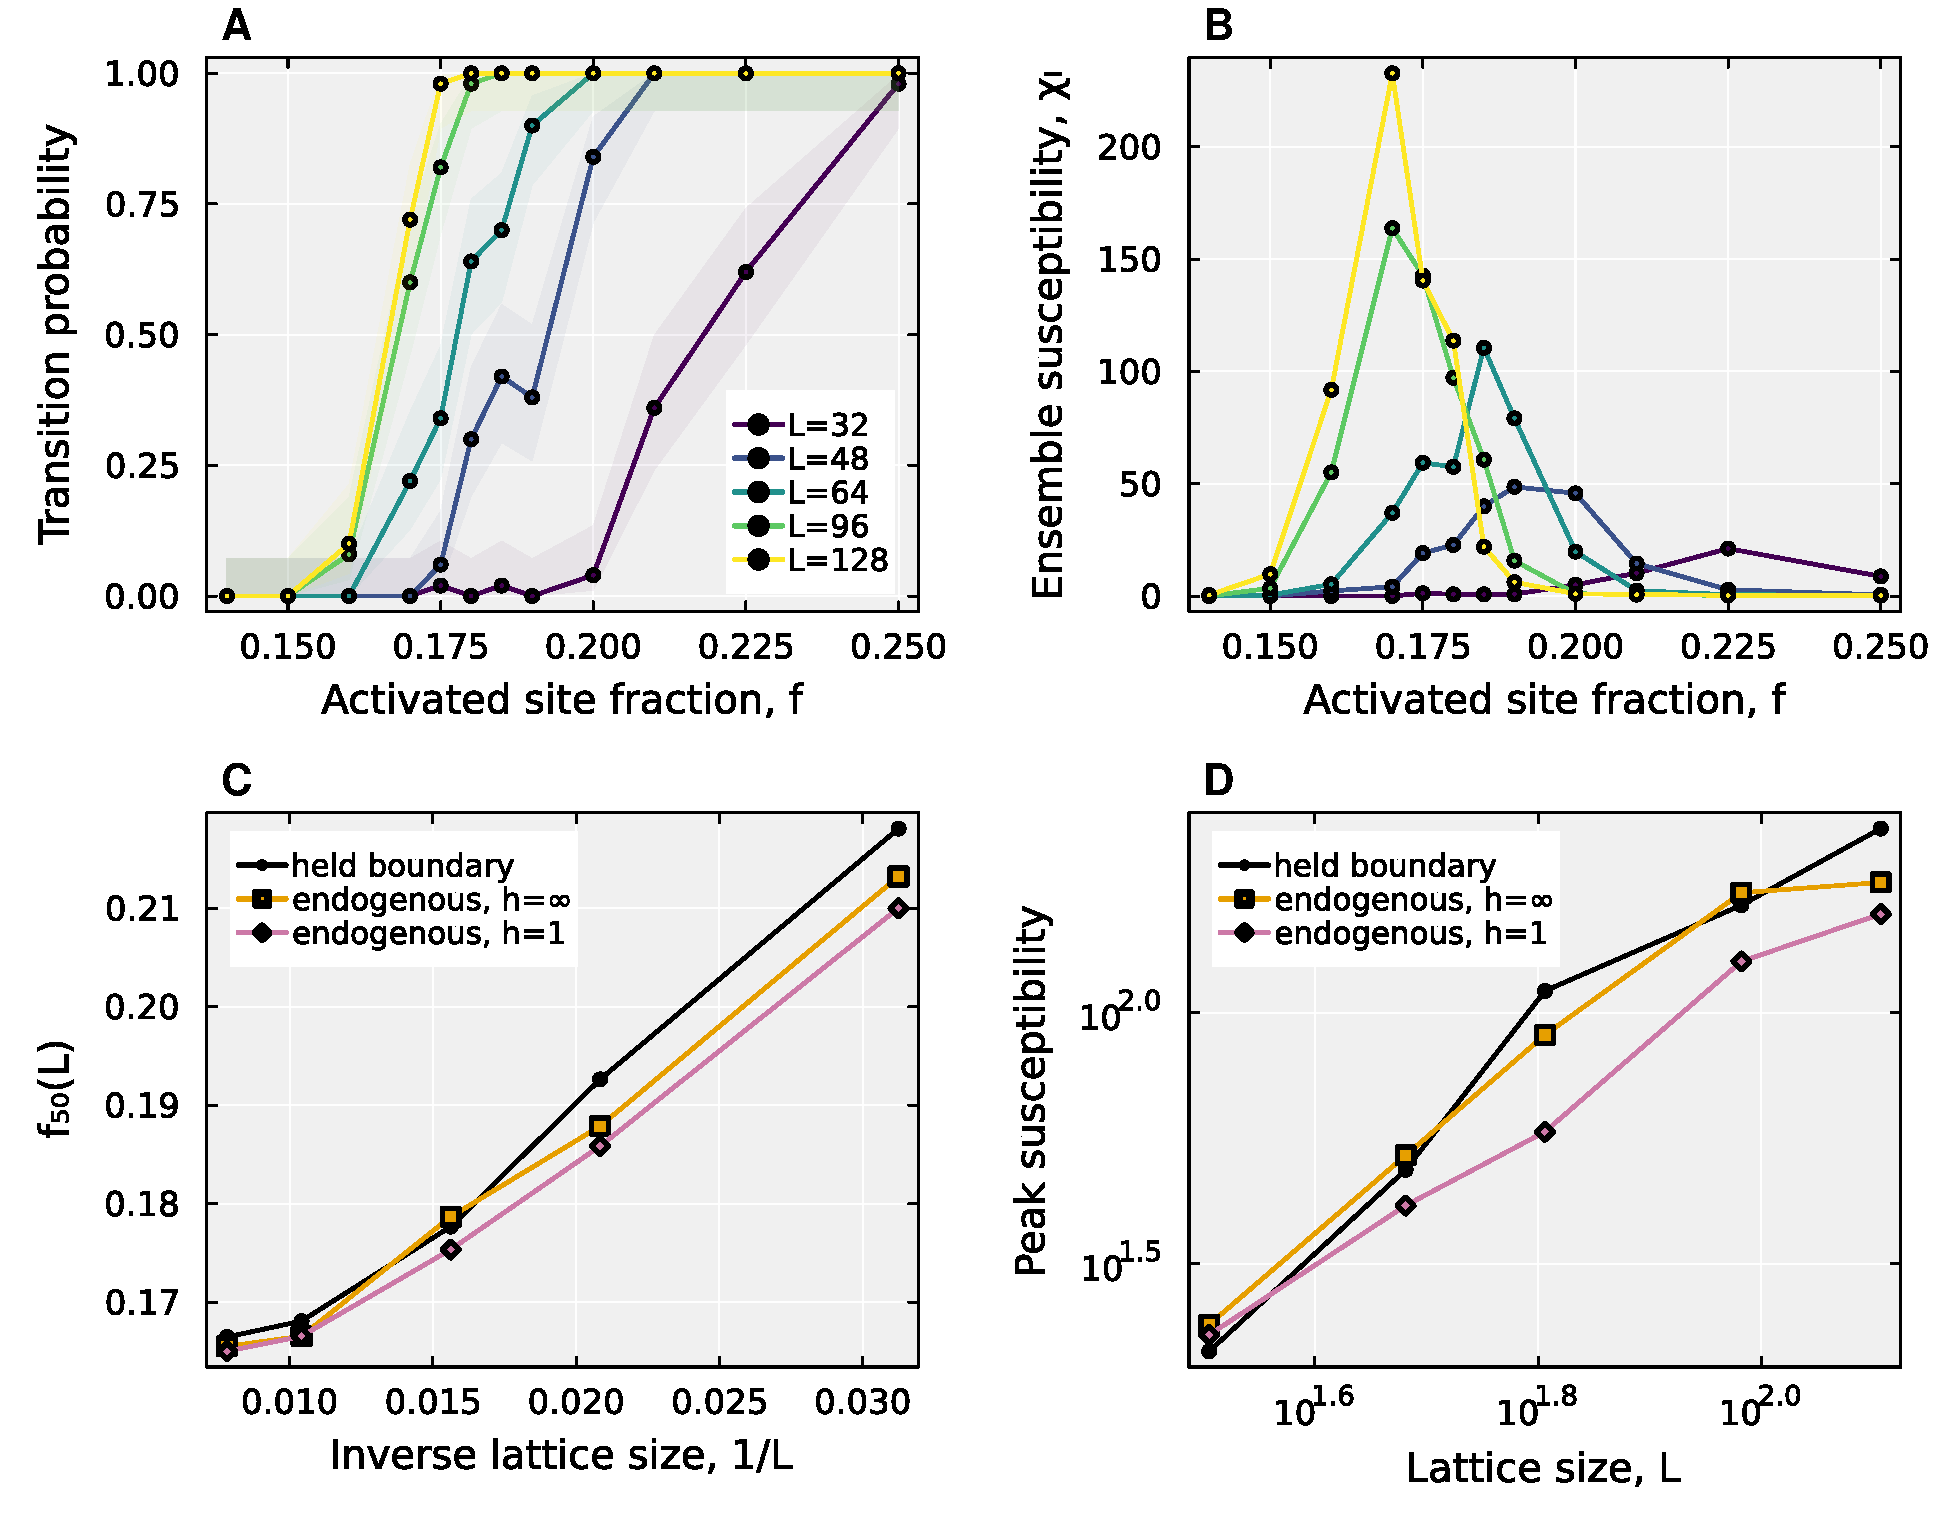
\includegraphics[width=0.97\linewidth]{figs/Fig3-FiniteSizeQuench.pdf}
  \caption{Effect of market size on the formation of a Sell majority over 50 starting
markets. \textbf{(A)}~Majority probability with edge traders kept in Hold;
bands are 95\% Wilson intervals. \textbf{(B)}~Variation between runs with
edge traders kept in Hold, measured as susceptibility: the variance of the
final 500-step mean Sell fraction multiplied by the number of interior
traders. \textbf{(C)}~Fraction $f_{50}(L)$ at which half the runs reached a
majority, estimated by interpolation for edge traders kept in Hold and for
two dealer capacities with edge traders responding to price.
\textbf{(D)}~Maximum susceptibility versus grid size on linear axes. Error
bars in (C,D) are 95\% intervals from resampling starting markets. Solid
lines connect tested values; dashed curves in (A) are logistic fits. No law
for the limit of indefinitely large grids was fitted.}
  \label{fig:finite-size}
\end{minipage}
\end{center}

\clearpage

\begin{center}
\begin{minipage}{\linewidth}
\captionsetup{type=figure,hypcap=false}
  \centering
  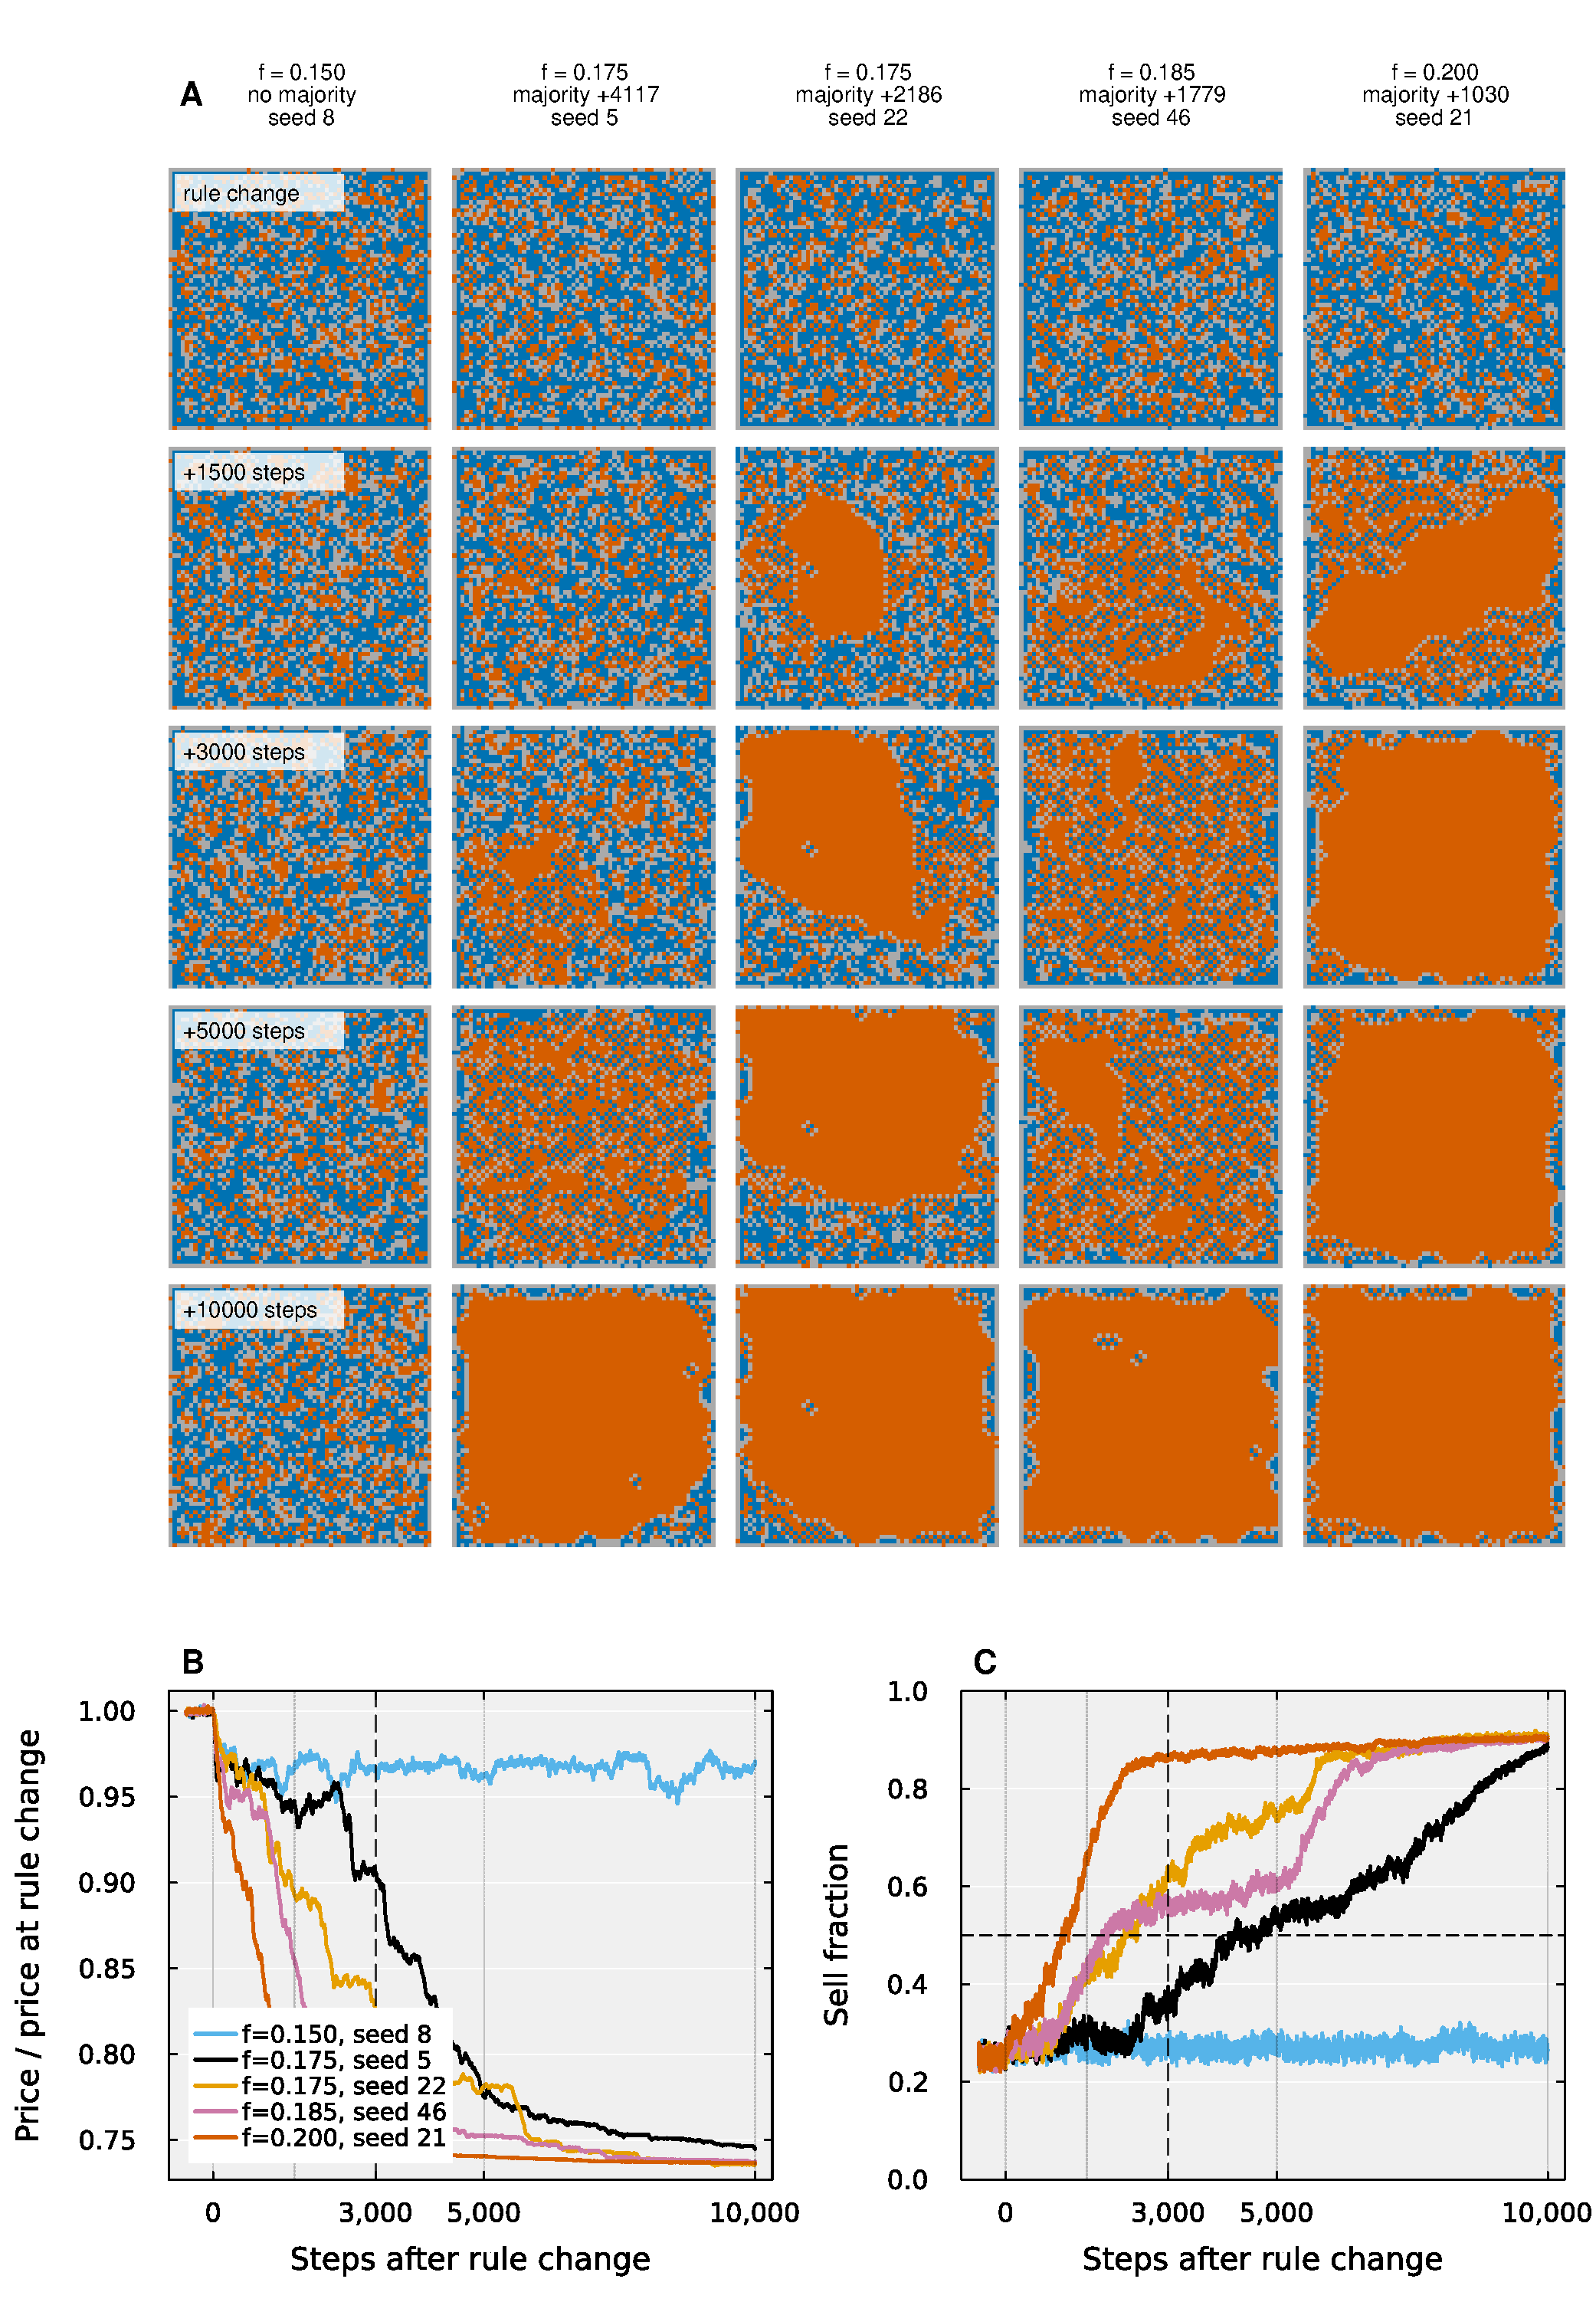
\includegraphics[width=0.98\linewidth]{figs/Fig4-DoseMarketPanels.pdf}
  \caption{How traders' decisions changed over time when different fractions received
the new rule, with edge traders responding to price and an unlimited dealer.
Blue, gray, and orange cells denote Buy, Hold, and Sell.
\textbf{(A)}~Decisions in five runs (columns) when the rule changed and
after 500, 1,500, and 3,000 steps (rows). From left to right, the runs
include a case without a majority at $f=0.15$, both outcomes at $f=0.175$,
and cases with a majority at $f=0.185$ and 0.20. Runs with a majority were
selected by proximity to their group's median time to a majority. Runs
without a majority were selected by proximity to their group's median final
Sell fraction. Selection preceded inspection of images. Seeds were 8, 5, 22,
46, and 21 from left to right. \textbf{(B)}~Price divided by its value when
the rule changed. \textbf{(C)}~Interior Sell fraction; the horizontal line
marks one-half. Vertical guides mark the four snapshots.}
  \label{fig:dose-panels}
\end{minipage}
\end{center}

\clearpage

\begin{center}
\begin{minipage}{\linewidth}
\captionsetup{type=figure,hypcap=false}
  \centering
  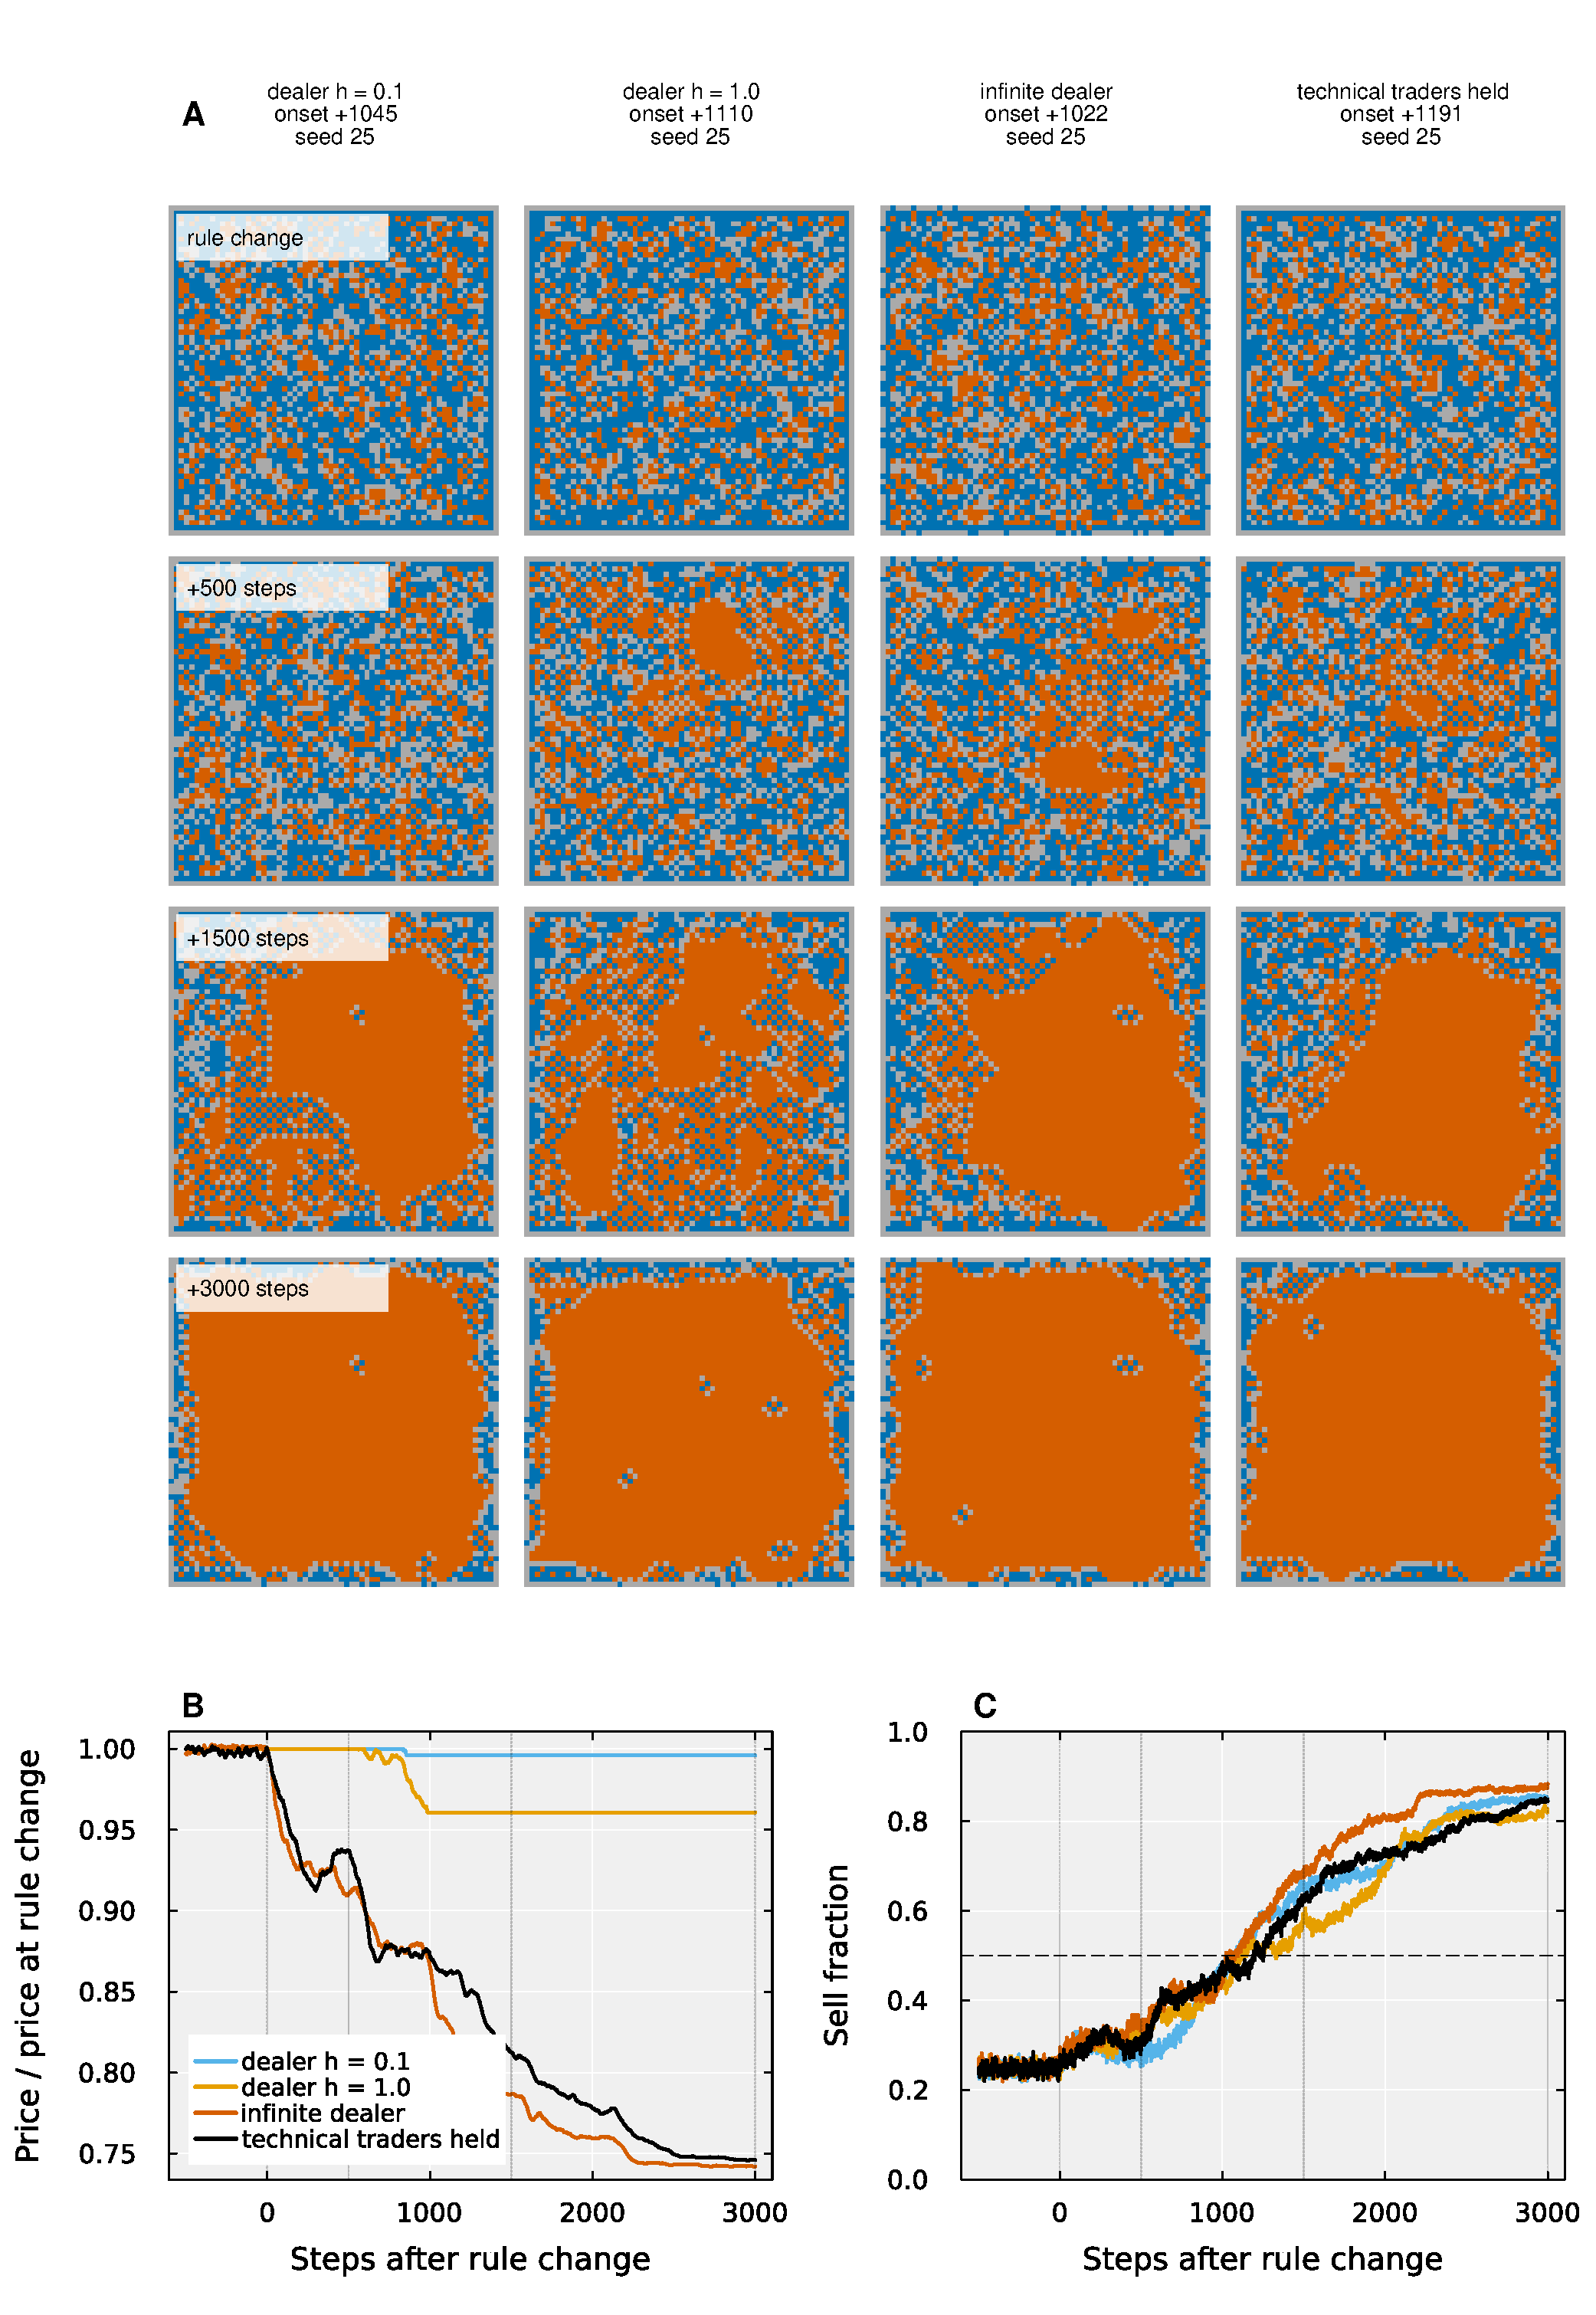
\includegraphics[width=0.92\linewidth]{figs/Fig5-DealerMarketPanels.pdf}
  \caption{How the same starting market developed with different dealer capacities at
$f=0.20$. \textbf{(A)}~Decisions under four conditions (columns) when the
rule changed and after 500, 1,500, and 3,000 steps (rows). The first three
columns allowed edge traders to respond to price, with dealer capacities
$h=0.1$, $h=1$, and $h=\infty$. The last kept edge traders in Hold with
$h=\infty$. Seed 25 was selected from runs that reached a majority at all
three capacities by minimizing the sum of distances from each capacity's
median time to a majority. Rows show the same elapsed times.
\textbf{(B)}~Price divided by its value when the rule changed.
\textbf{(C)}~Interior Sell fraction. Keeping edge traders in Hold prevented
price from influencing decisions inside the grid; trades and price changes
were still calculated. This example follows one starting market, while the
full comparison measures outcomes across starting markets
(Fig.~\ref{fig:reservoir}).}
  \label{fig:dealer-panels}
\end{minipage}
\end{center}

\clearpage

\begin{center}
\begin{minipage}{\linewidth}
\captionsetup{type=figure,hypcap=false}
  \centering
  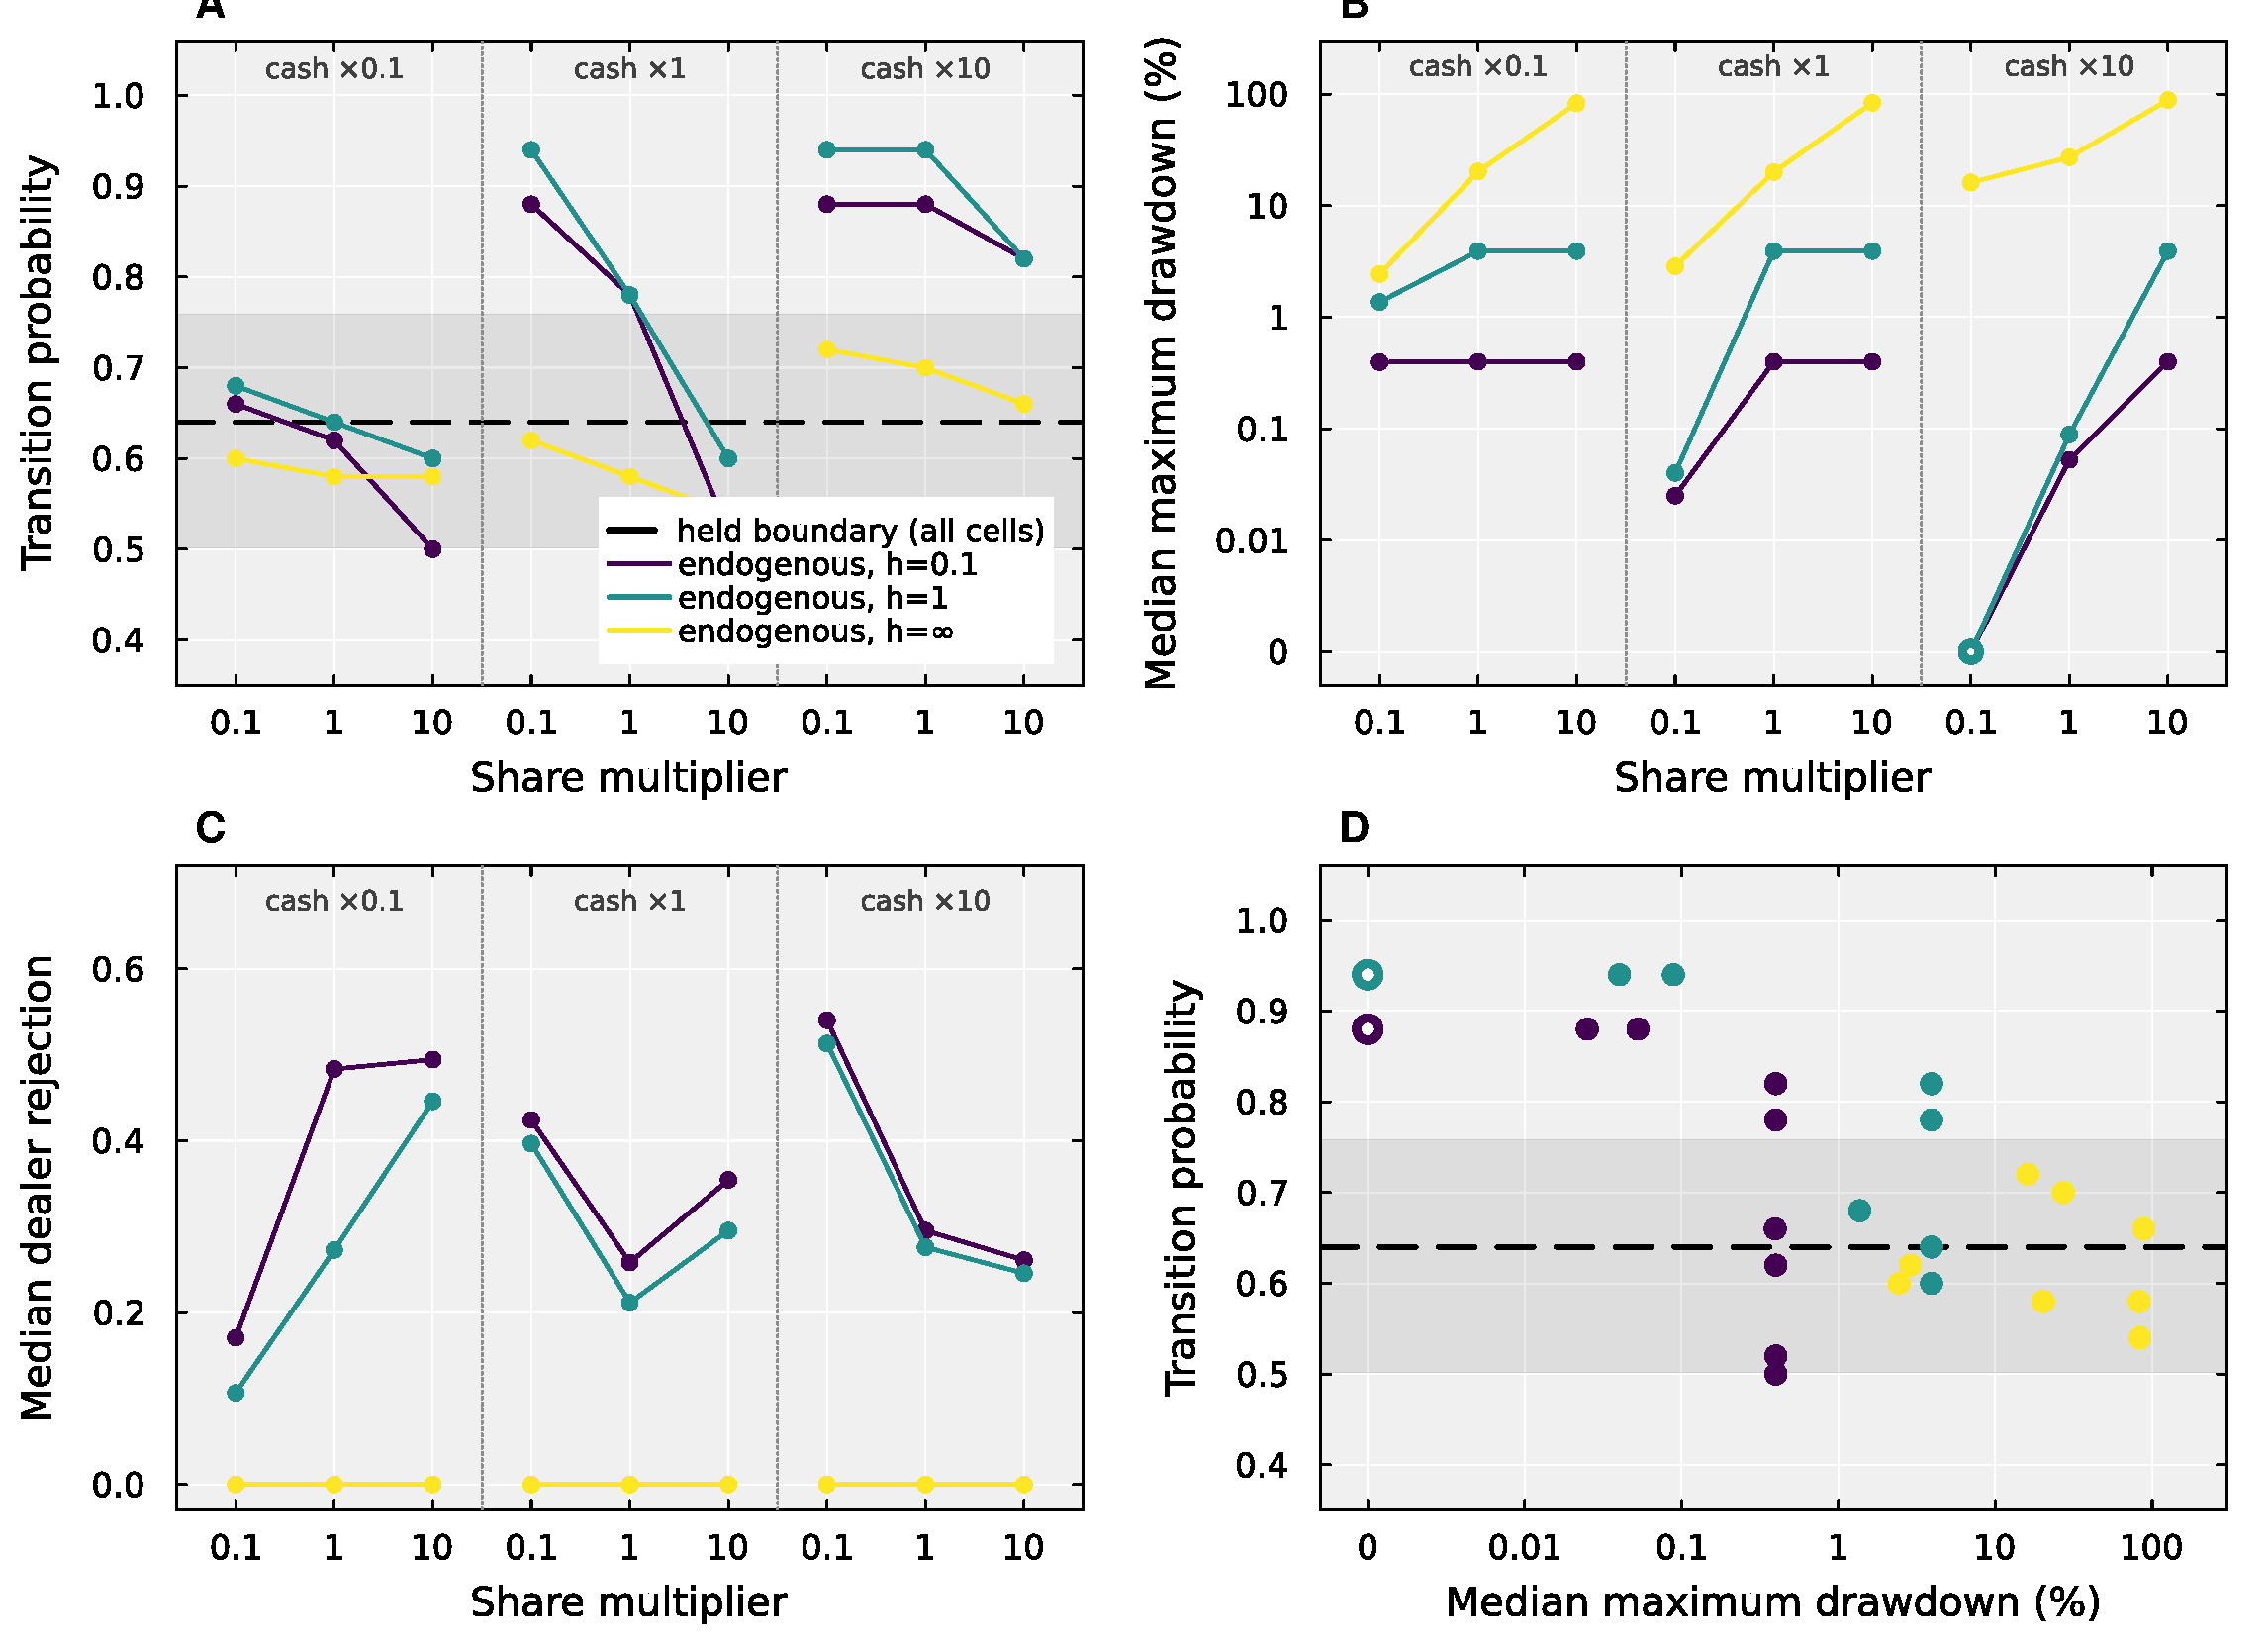
\includegraphics[width=0.99\linewidth]{figs/Fig6-BalanceSheetQuench.pdf}
  \caption{Effects of changing traders' cash and shares when the new decision rule was
introduced, with edge traders responding to price, $f=0.18$, and 50 starting
markets. In A to C, the nine combinations are grouped by cash multiplier,
with share multiplier on the axis and a separate series for each dealer
capacity. \textbf{(A)}~Probability of a Sell majority. The dashed line and
band give the probability and its 95\% Wilson interval with edge traders
kept in Hold, which were identical in all nine combinations because resource
changes could not affect decisions. \textbf{(B)}~Median maximum drawdown on
a logarithmic axis. Medians of exactly zero appear at the axis floor with
open markers. \textbf{(C)}~Median fraction of orders backed by trader cash
or shares that the dealer rejected. \textbf{(D)}~Majority probability
against median maximum drawdown for all 27 combinations of cash, shares, and
dealer capacity with edge traders responding to price. The axis and zero
markers follow B, and the reference probability with edge traders kept in
Hold is repeated.}
  \label{fig:balance-sheet}
\end{minipage}
\end{center}
